\subsection{Memcached}
\label{sec:mcd}

\begin{figure*}
\centering
%\vspace*{-0.3cm}  
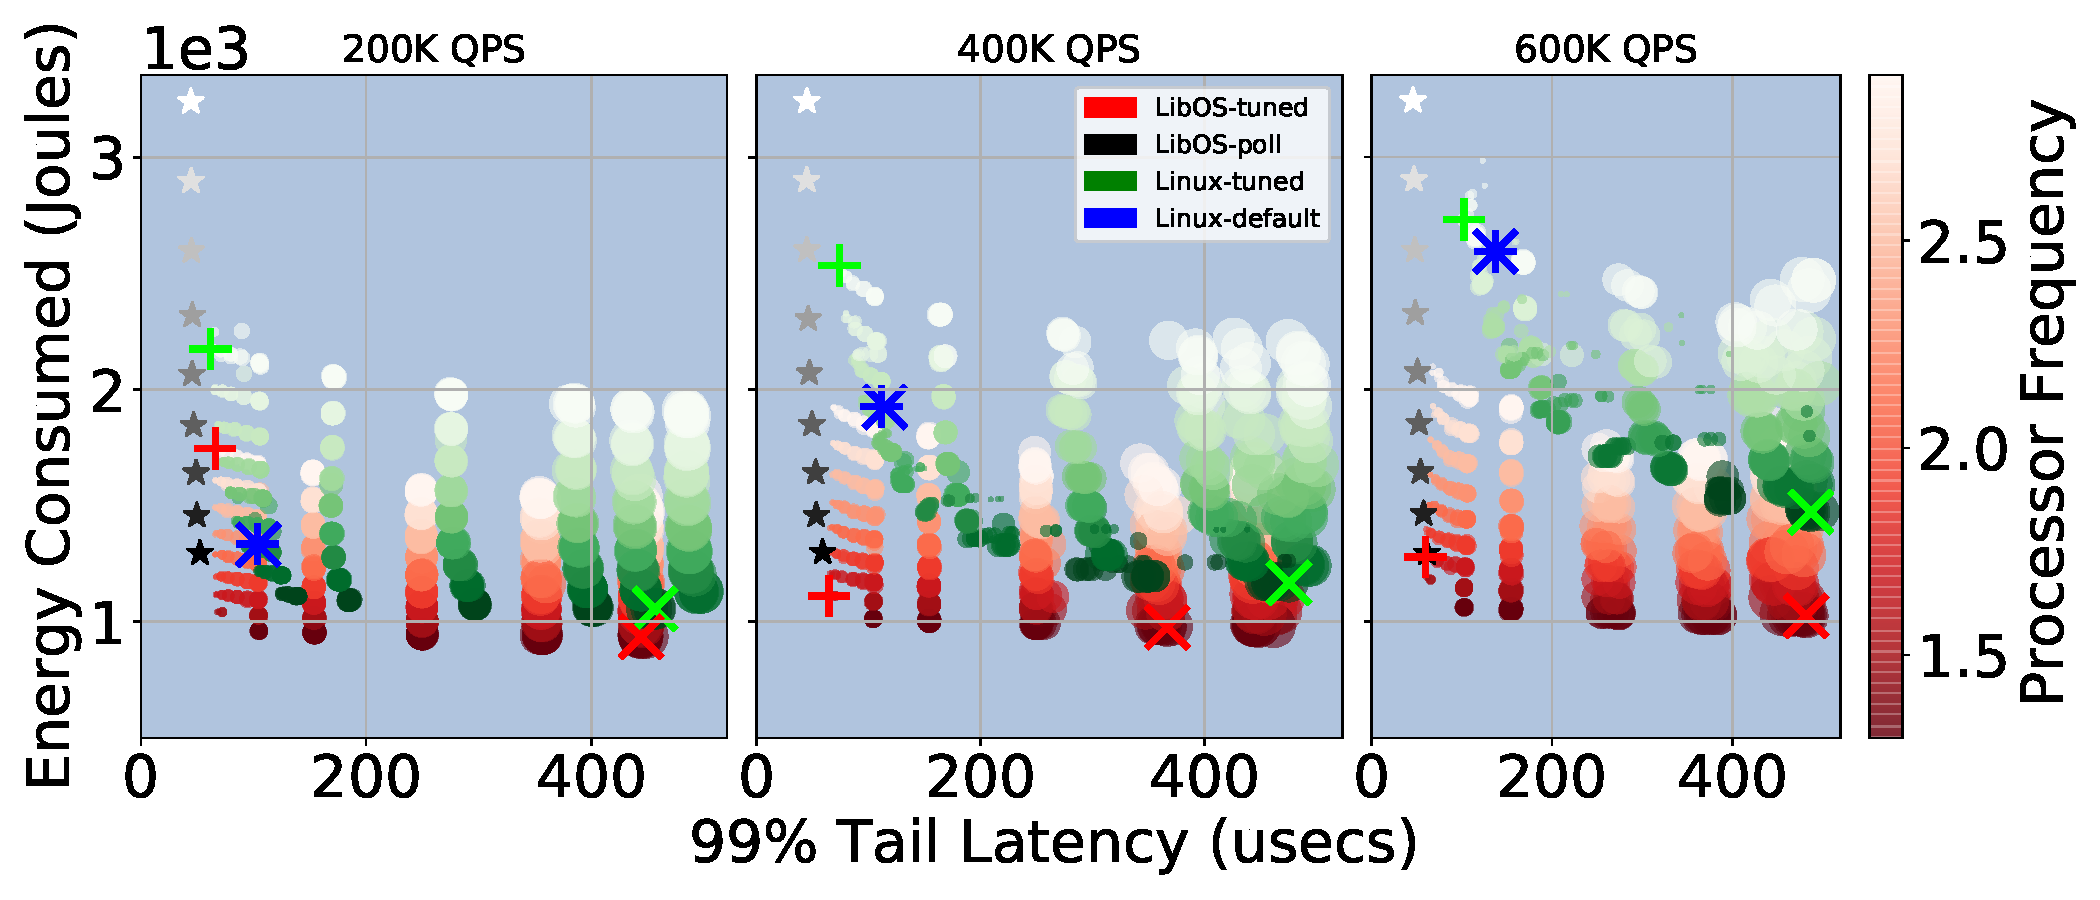
\includegraphics[width=1\textwidth]{figures/mcd_overview}
\caption[]
%{\small 
{Overview of memcached experiments across 200K, 400K, and 600K QPS. Each circle represents an experimental run of tuning ITR-delay and DVFS. The larger the size of a circle equates to larger ITR-delay value. The darkening of color gradient indicates slowing down processor frequency. The \textbf{x} indicate lowest energy consumption. The \textbf{+} indicate lowest tail latency.}
\label{fig:mcd_overview}
\end{figure*}

Memcached~\cite{mcd} is a multi-threaded workload that runs on all 16 cores of any one of our server nodes. It consists of an unloaded client node running mutilate~\cite{mutilate}. This client (1) coordinates with five other mutilate agent nodes in order to generate requests to the server and (2) measures tail latency of all requests made. All five agent nodes are 16-core machines, whereby each core creates 16 connections, for a total of 1280 connections. This setup is able to saturate the single 16-core server\footnote{Mutilate is configured to pipeline up to four connections to further increase its request rate.}. Our library OS uses a re-implemented version of memcached, written to the OS's interfaces, which supports the standard memcached binary protocol. To alleviate lock contention, an RCU hashtable is used to store key-value pairs. We run a representative load from Facebook~\cite{workloadanalysisfacebook} (ETC) which represents the highest capacity deployment. It uses 20 - 70 byte keys and 1 byte to 1 KB values and contains 75\% GET requests.

\begin{figure}
%\centering
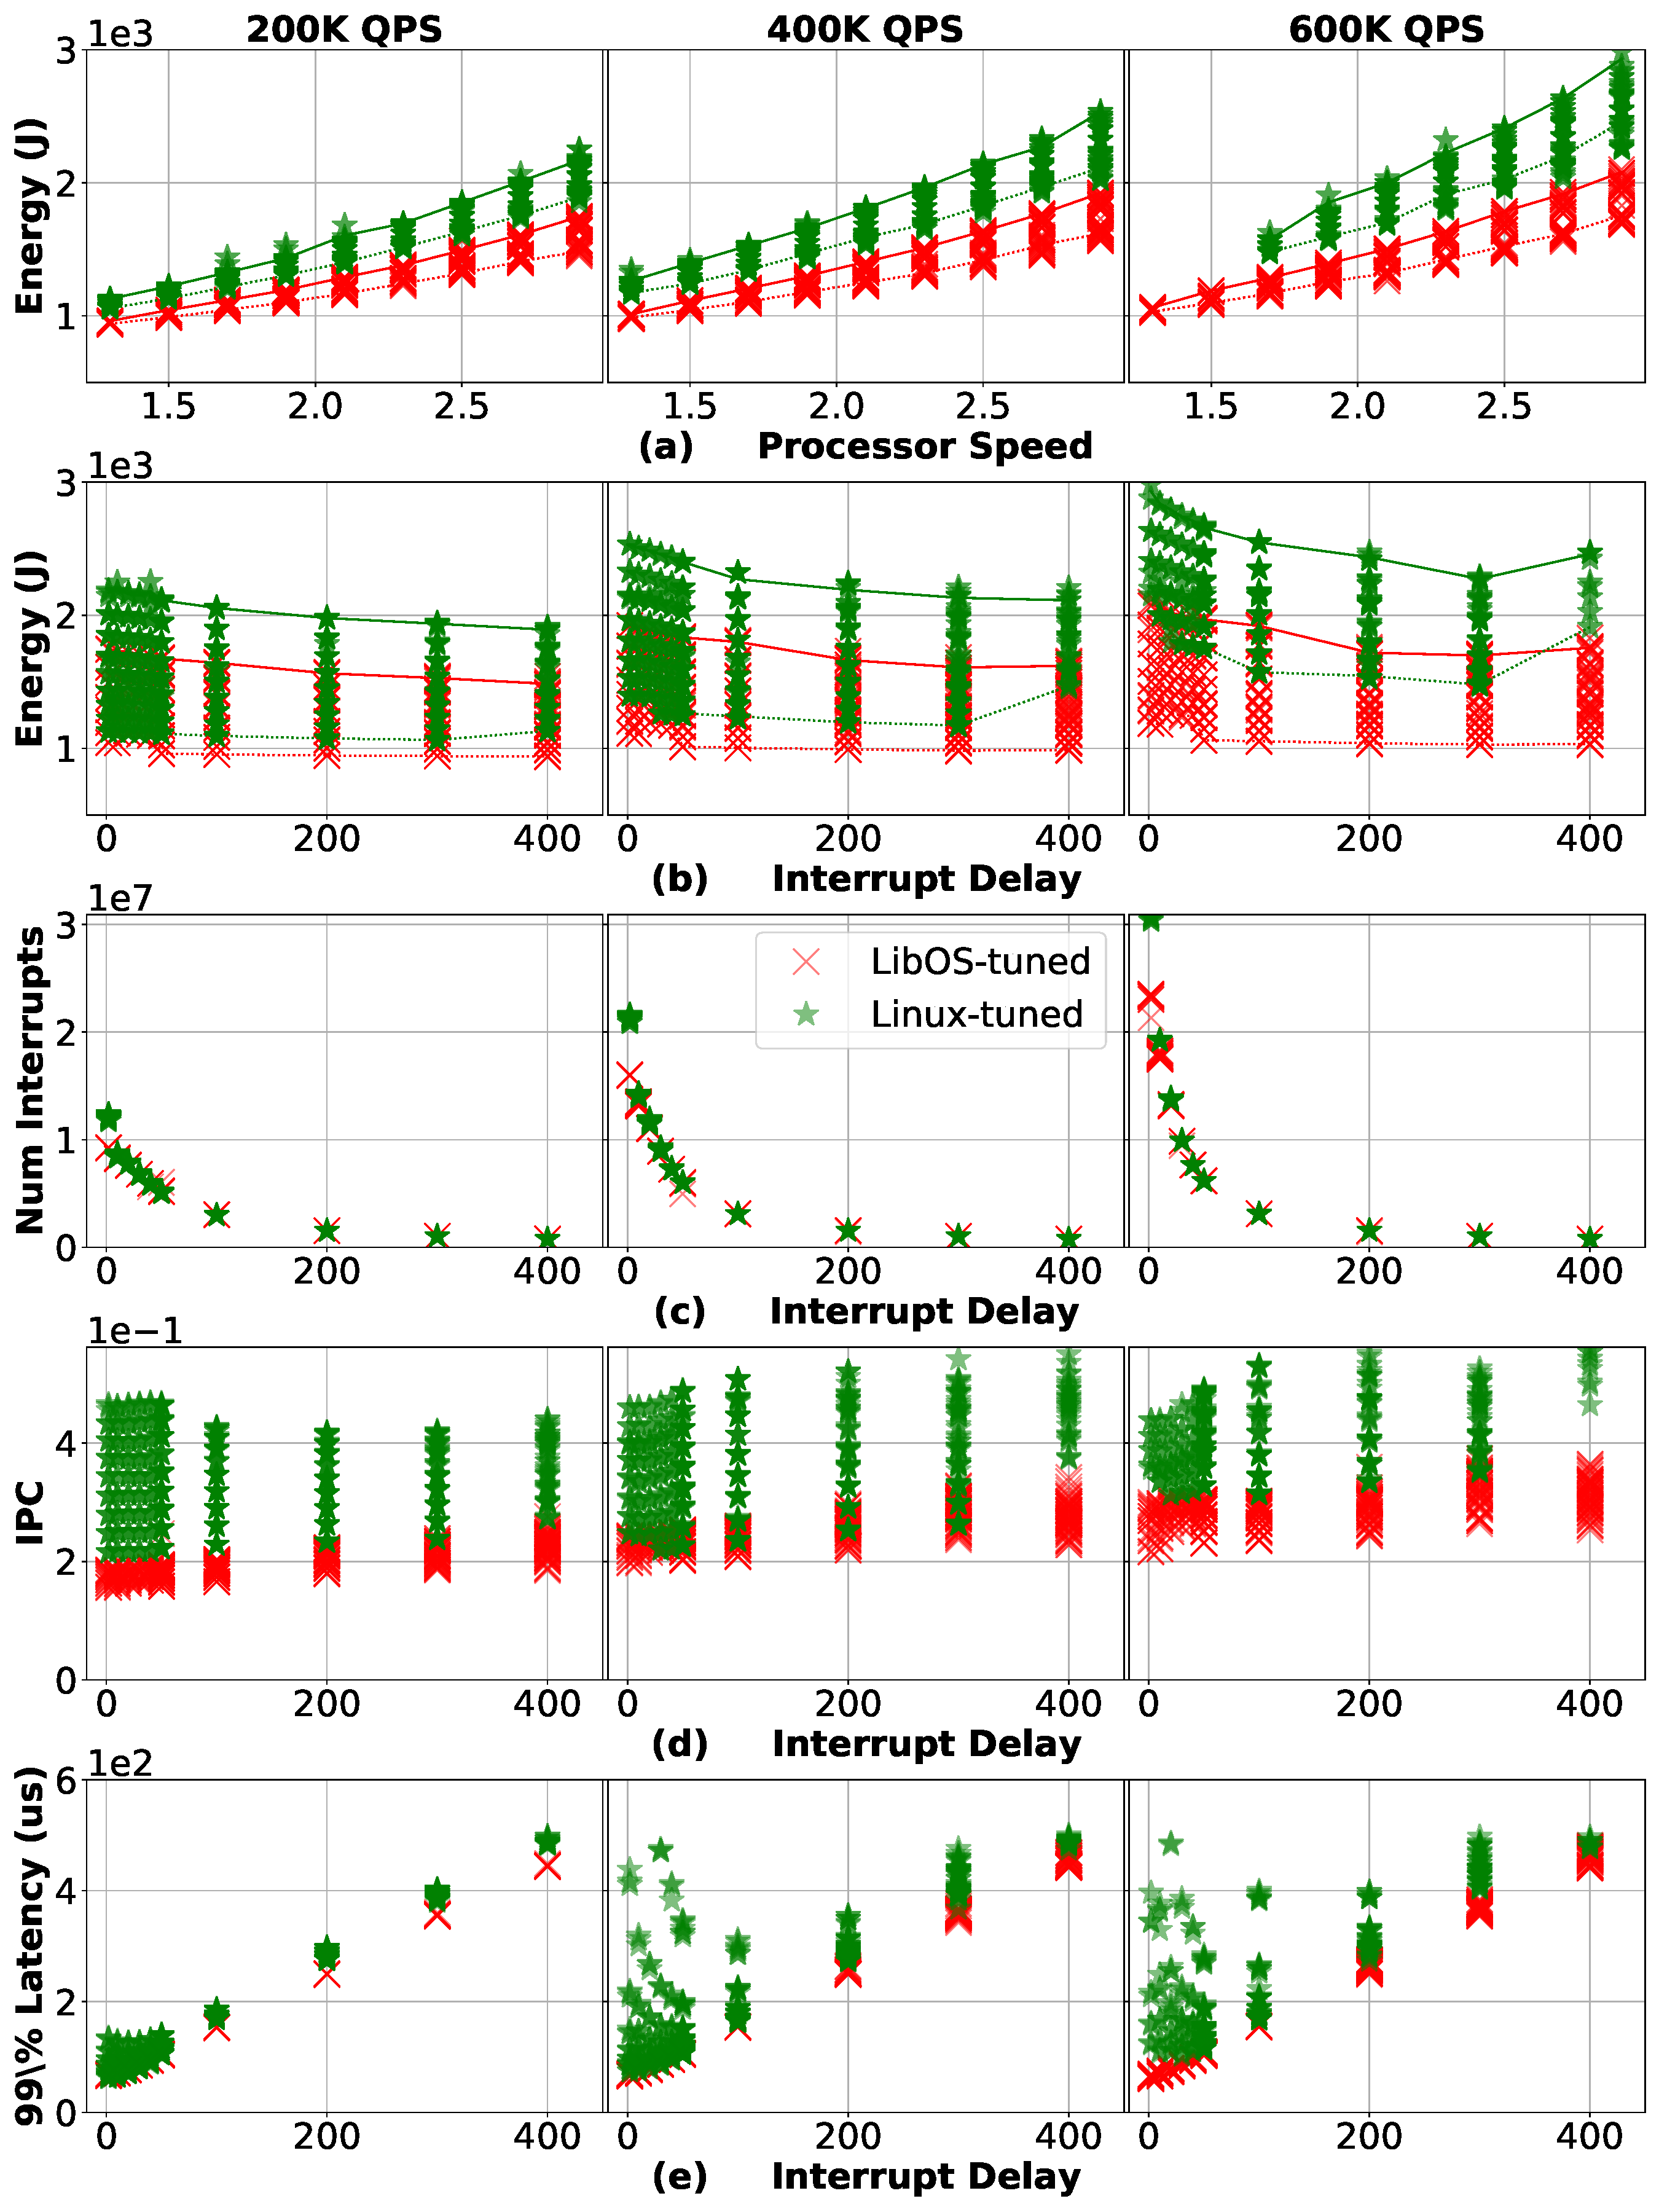
\includegraphics[width=0.5\textwidth]{figures/mcd_detail_1}
%\hspace*{-10.0cm} 
%\vspace*{-1.0cm}  
\caption[]{}
\label{fig:mcd_detail_1}
\end{figure}

\begin{figure}
%\centering
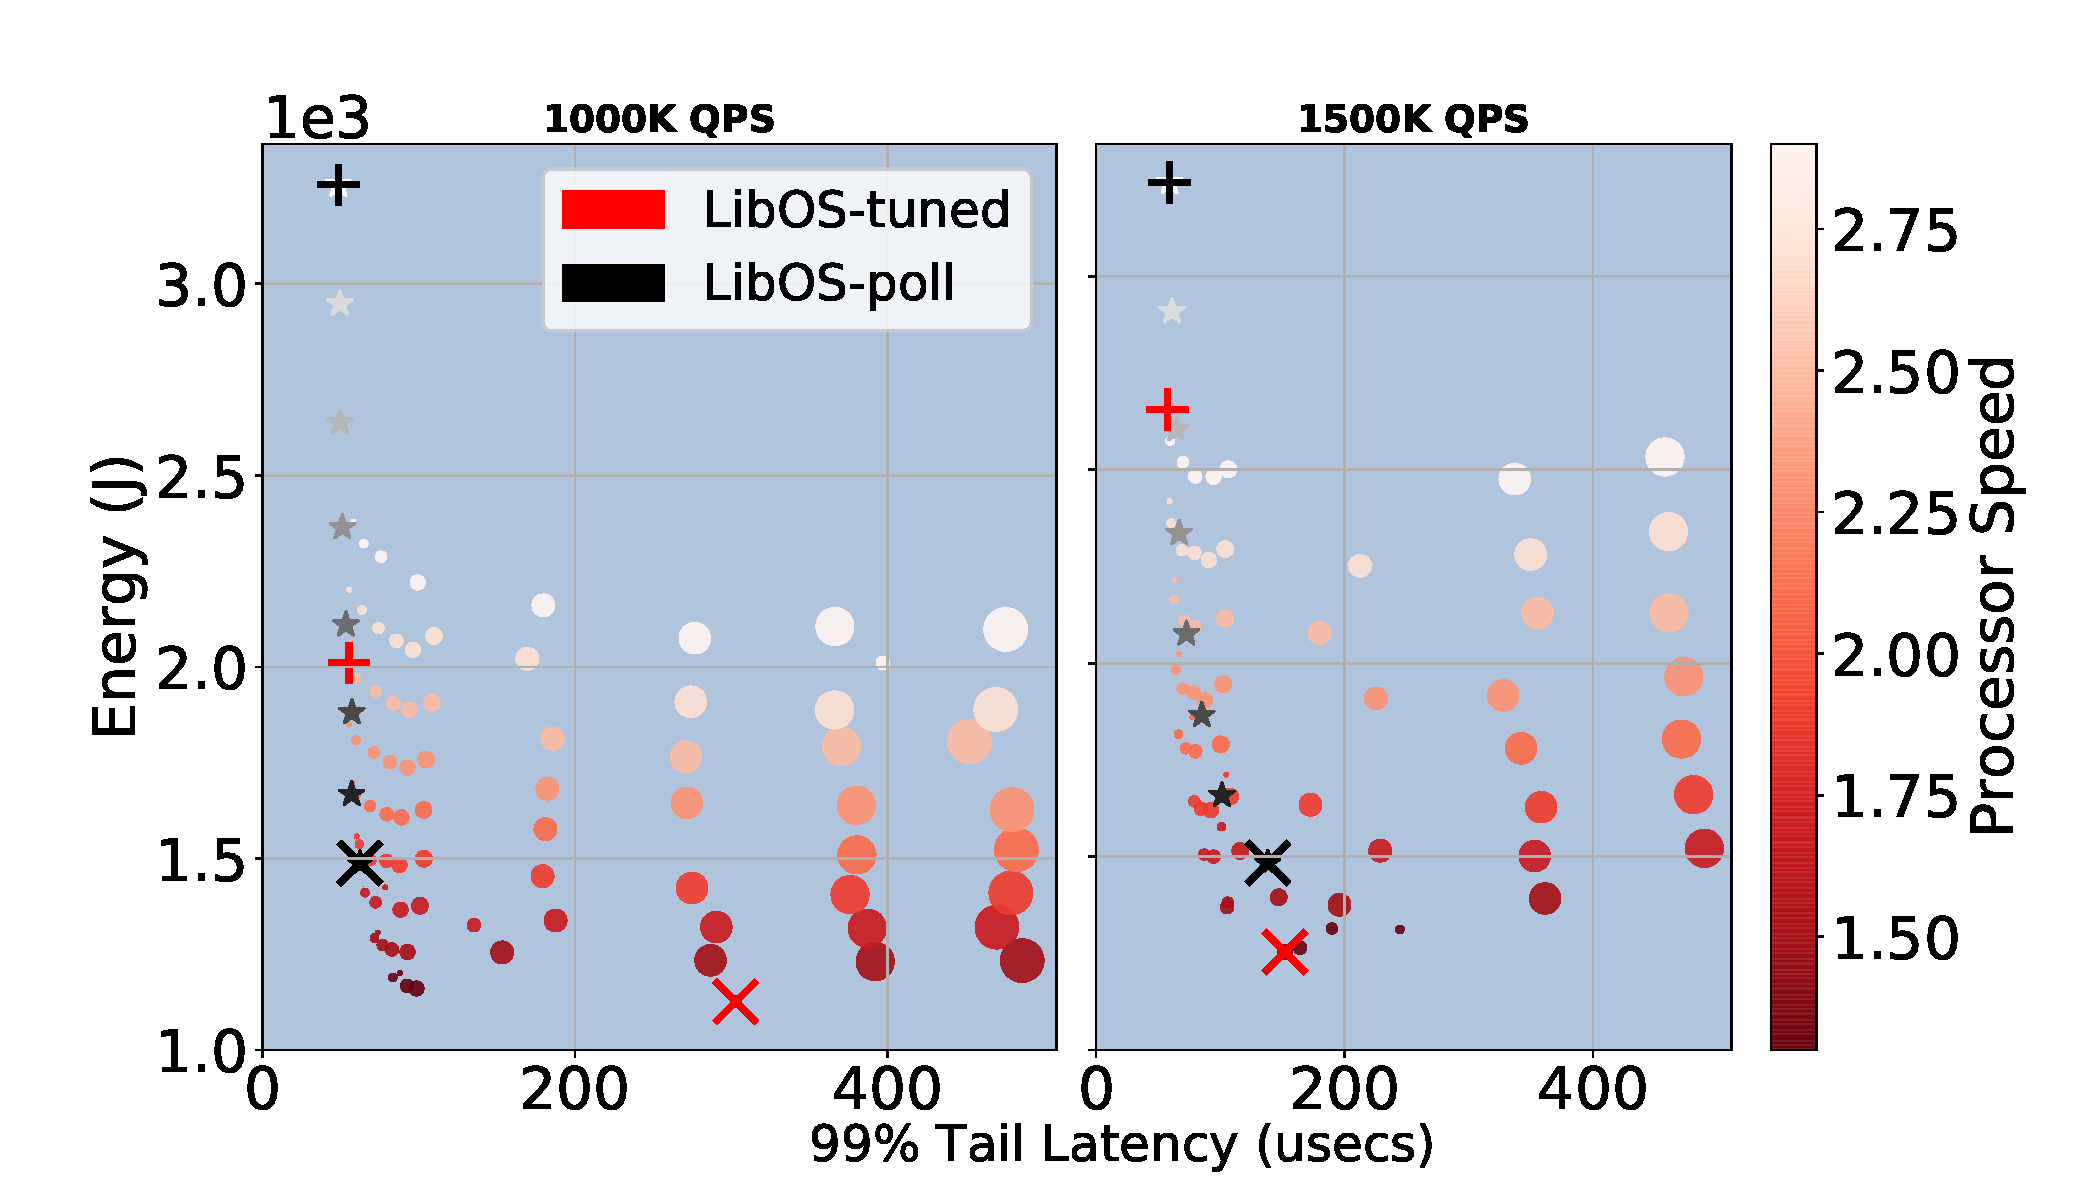
\includegraphics[width=0.5\textwidth]{figures/mcd_overview2}
%\vspace*{-1.0cm}  
\caption[]{}
\label{fig:mcd_overview2}
\end{figure}

% 200000 ebbrt_tuned 
%  	 SLOW-ITR-diff-Min-Max-DVFS= 702.25 J
%  	 FAST-ITR-diff-Min-Max-DVFS= 544.91 J

% 200000 linux_tuned 
%  	 SLOW-ITR-diff-Min-Max-DVFS= 1041.8 J
%  	 FAST-ITR-diff-Min-Max-DVFS= 760.76 J

% 400000 ebbrt_tuned 
%  	 SLOW-ITR-diff-Min-Max-DVFS= 809.36 J
%  	 FAST-ITR-diff-Min-Max-DVFS= 632.57 J

% 400000 linux_tuned 
%  	 SLOW-ITR-diff-Min-Max-DVFS= 1135.93 J
%  	 FAST-ITR-diff-Min-Max-DVFS= 644.14 J

% 600000 ebbrt_tuned 
%  	 SLOW-ITR-diff-Min-Max-DVFS= 891.97 J
%  	 FAST-ITR-diff-Min-Max-DVFS= 723.47 J

% 600000 linux_tuned 
%  	 SLOW-ITR-diff-Min-Max-DVFS= 706.79 J
%  	 FAST-ITR-diff-Min-Max-DVFS= 547.11 J

\subsubsection{Finding-1: Slowing down processor has better performance-energy trade-offs for memcached than using sleep states.} \label{sec:f1} Figure~\ref{fig:mcd_detail_1}(b) shows that even though interrupts are slowed down, the energy differences within each interrupt delay rate is largely determined by the differences in processor speeds. The bold lines connect the mean energy use of each interrupt delay rate whereby processor speed is fastest while the dotted lines connect the mean energy use where processor speed is slowest. Compared to figure~\ref{fig:mcd_detail_1}(a), where the processor speeds are shown on the x-axis and the differences in energy use is caused by different interrupt delay rates, we find that reducing energy use by slowing down the \textit{processor} is 2-10X more effective than by slowing down \textit{interrupt} rates (i.e. increased potential for using sleep states) across different QPS rates and OS structure as well. We believe the main reason is that memcached workloads are bursty with multiple requests pipelined onto multiple cores, therefore the system as whole is always busy with work. This renders potential energy savings by prolonged periods of idleness not as effective as slowing down the processor itself. It should also be noted that Linux at 600K QPS has a smaller energy gap at an interrupt delay rate of \SI{400}{\micro s} due to the fact that SLA violations already started to occur at faster processor speeds.
% 200000 ebbrt_tuned 
%  	 SLOW-DVFS-diff-Min-Max-ITR= 21.11 J
%  	 FAST-DVFS-diff-Min-Max-ITR= 260.41 J
%  	 FAST/SLOW= 12.3359
% 200000 linux_tuned 
%  	 SLOW-DVFS-diff-Min-Max-ITR= 70.94 J
%  	 FAST-DVFS-diff-Min-Max-ITR= 277.91 J
%  	 FAST/SLOW= 3.9175
% 400000 ebbrt_tuned 
%  	 SLOW-DVFS-diff-Min-Max-ITR= 25.48 J
%  	 FAST-DVFS-diff-Min-Max-ITR= 302.86 J
%  	 FAST/SLOW= 11.8862
% 400000 linux_tuned 
%  	 SLOW-DVFS-diff-Min-Max-ITR= 90.47 J
%  	 FAST-DVFS-diff-Min-Max-ITR= 420.31 J
%  	 FAST/SLOW= 4.6458
% 600000 ebbrt_tuned 
%  	 SLOW-DVFS-diff-Min-Max-ITR= 30.19 J
%  	 FAST-DVFS-diff-Min-Max-ITR= 325.17 J
%  	 FAST/SLOW= 10.7708
% 600000 linux_tuned 
%  	 SLOW-DVFS-diff-Min-Max-ITR= 92.84 J
%  	 FAST-DVFS-diff-Min-Max-ITR= 471.21 J
%  	 FAST/SLOW= 5.0755
\subsubsection{Finding-2: Ineffectiveness of sleep state energy savings at slow processor speeds.}
\label{sec:f2}
Figure~\ref{fig:mcd_detail_1}(a) shows that as a processor slows down, the energy savings from slow downing down interrupt rates also decreases (larger energy gap to smaller energy gap). Bold lines indicate the mean energy use at fastest interrupt rate, while dotted lines indicate mean energy use at slowest interrupt rate. 

First, we find that across the QPS loads and the two OSes, the average energy savings from slowing down interrupt rates at the \textit{slowest} processor speed is around \SI{52}{\joule} while at the \textit{fastest} processor speed we get a average energy savings of around \SI{342}{\joule}. Referring back to figure~\ref{fig:timeline}, the effect of slowing down the processor results in the lengthening of the application and OS work in memcached, thereby reducing the benefits of prolonged idle periods to take advantage of energy savings by sleep states, this is also further exacerbated by the SLA requirements which results in a strict time budget each request must adhere to. 

%Second, we find that in the libOS, slowing down interrupt rates at the fastest processor speed results in around 11X better energy savings over the slowest processor speed. Similarly we find the same benefits in Linux, however, the energy savings are only around 4X better.

\subsubsection{Finding-3: OS path length efficiency and polling} \label{sec:f3}
Even though figure~\ref{fig:mcd_overview} indicates the libOS uses lower energy than Linux across all QPS loads, we find that in both figures~\ref{fig:mcd_detail_1}(a)(b), Linux is always able to save more energy (1.02X to 3.6X) by slowing down processor and interrupt rates than the libOS. We believe this more a result of the base efficiency of libOS' (figure~\ref{fig:mcd_detail_1}(d) shows libOS using ~2.5X fewer instructions than Linux) and optimized OS path lengths (figure~\ref{fig:mcd_overview2} shows libOS can support higher QPS loads than Linux). This is further supported by the \textit{vertical-ness} of the libOS datapoints in figure~\ref{fig:mcd_overview}, which largely shows the ineffectiveness of slowing down the processor in causing a increase in the tail latency. We can see the opposite of this behavior in Linux where at 600K QPS, it is approach 75\% of the peak QPS it can support, there is a clear trade-off between slowing down processor speeds and an increase in tail latency (higher latency points tend to have darker gradient color). In figure~\ref{fig:mcd_overview2}, memcached is scaled higher to 1500K QPS, which is 75\% of the libOS' peak QPS it can support, at this QPS rate we can begin to see the processor speed and tail latency trade-off.

\textbf{Polling - TODO}
\subsubsection{Finding-4: Fast interrupt rates induces behavior for low tail latency at high energy use.} \label{sec:f4}


\subsubsection{Finding-5: Slowing down both processor and interrupt rate} \label{sec:f5}